\documentclass{article}
\usepackage{amsmath, amssymb, graphicx, tikz}
\usetikzlibrary{positioning}
\usepackage{hyperref}


\title{Lecture Notes: Autoencoders}
\author{Your Name}
\date{\today}

\begin{document}

\maketitle

\section{Introduction to Autoencoders}

Autoencoders are a class of neural networks designed to learn efficient representations of data, typically for dimensionality reduction or feature extraction. The architecture consists of two main components: an encoder and a decoder. The encoder compresses the input into a latent-space representation, while the decoder reconstructs the input from this latent space. Autoencoders are widely used in tasks such as data denoising, dimensionality reduction, and generative modeling.

\section{Autoencoder Architecture}

An autoencoder's basic structure can be illustrated as follows:

\begin{figure}[h]
    \centering
    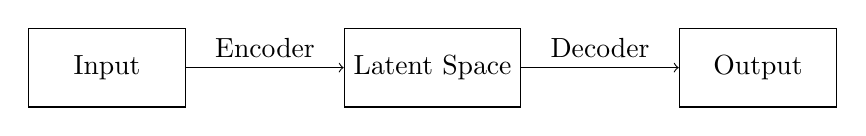
\begin{tikzpicture}
    % Encoder
    \node[draw, minimum width=2cm, minimum height=1cm] (input) {Input};
    \node[draw, minimum width=2cm, minimum height=1cm, right=2cm of input] (hidden) {Latent Space};
    \node[draw, minimum width=2cm, minimum height=1cm, right=2cm of hidden] (output) {Output};

    % Arrows
    \draw[->] (input) -- node[above] {Encoder} (hidden);
    \draw[->] (hidden) -- node[above] {Decoder} (output);
    \end{tikzpicture}
    \caption{Basic architecture of an autoencoder.}
    \label{fig:autoencoder}
\end{figure}

\subsection{Mathematical Representation}

Given an input vector \( \mathbf{x} \), the encoder maps it to a latent representation \( \mathbf{z} \) using a function \( f_\theta \):
\[
\mathbf{z} = f_\theta(\mathbf{x})
\]
The decoder then maps \( \mathbf{z} \) back to the reconstructed input \( \mathbf{\hat{x}} \) using another function \( g_\phi \):
\[
\mathbf{\hat{x}} = g_\phi(\mathbf{z})
\]
The goal is to minimize the reconstruction error, often measured by Mean Squared Error (MSE):
\[
\text{MSE} = \frac{1}{n} \sum_{i=1}^{n} (\mathbf{x}_i - \mathbf{\hat{x}}_i)^2
\]

\section{Types of Autoencoders}

\subsection{Vanilla Autoencoder}

A vanilla autoencoder consists of a simple feedforward network where the number of neurons in the input layer equals the number of neurons in the output layer. The network is trained to minimize the difference between the input and the output.

\begin{figure}[h]
    \centering
    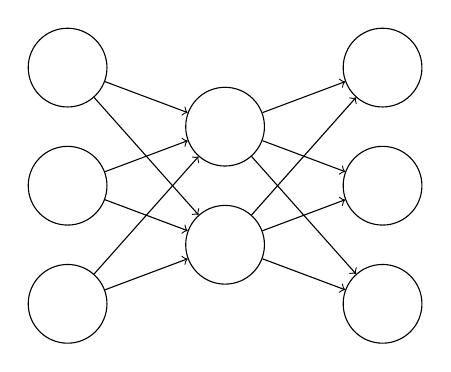
\begin{tikzpicture}
    % Layers
    \node[draw, circle, minimum size=1cm] (i1) at (0,0) {};
    \node[draw, circle, minimum size=1cm] (i2) at (0,-1.5) {};
    \node[draw, circle, minimum size=1cm] (i3) at (0,-3) {};
    
    \node[draw, circle, minimum size=1cm] (h1) at (2,-0.75) {};
    \node[draw, circle, minimum size=1cm] (h2) at (2,-2.25) {};
    
    \node[draw, circle, minimum size=1cm] (o1) at (4,0) {};
    \node[draw, circle, minimum size=1cm] (o2) at (4,-1.5) {};
    \node[draw, circle, minimum size=1cm] (o3) at (4,-3) {};

    % Connections
    \foreach \i in {1,2,3}
        \foreach \j in {1,2}
            \draw[->] (i\i) -- (h\j);

    \foreach \i in {1,2}
        \foreach \j in {1,2,3}
            \draw[->] (h\i) -- (o\j);
    \end{tikzpicture}
    \caption{Vanilla Autoencoder with one hidden layer.}
    \label{fig:vanilla_ae}
\end{figure}

\subsection{Sparse Autoencoder}

Sparse autoencoders impose a sparsity constraint on the hidden units, encouraging the network to learn a more efficient and robust set of features. This is typically achieved by adding a penalty to the loss function that enforces sparsity.

\begin{itemize}
    \item **Motivation:** Sparse autoencoders are particularly useful for feature extraction, where the learned features are sparse and informative, making them suitable for transfer learning in tasks such as classification.
    \item **Example:** In image recognition, sparse features learned by an autoencoder can be transferred to a classifier to improve its performance.
\end{itemize}

\subsubsection{Mathematical Formulation}

The loss function for a sparse autoencoder can be written as:
\[
L = \frac{1}{n} \sum_{i=1}^{n} \left[ (\mathbf{x}_i - \mathbf{\hat{x}}_i)^2 + \lambda \sum_{j=1}^{m} KL(\rho || \hat{\rho}_j) \right]
\]
where \( KL(\rho || \hat{\rho}_j) \) is the Kullback-Leibler divergence between the desired average activation \( \rho \) and the actual average activation \( \hat{\rho}_j \).

\subsection{Denoising Autoencoder}

Denoising autoencoders are trained to reconstruct the original input from a corrupted version of the input. This training method enhances the autoencoder's robustness to noise, making it effective for tasks like image denoising.

\subsubsection{Training Process}

During training, noise is added to the input, and the network is trained to minimize the reconstruction error between the output and the original (clean) input.

\begin{figure}[h]
    \centering
    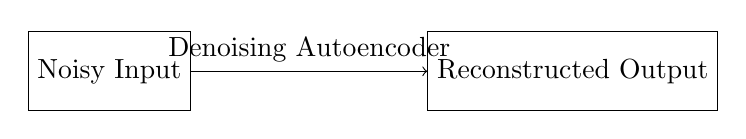
\begin{tikzpicture}
    % Input with noise
    \node[draw, minimum width=2cm, minimum height=1cm] (input) {Noisy Input};
    \node[draw, minimum width=2cm, minimum height=1cm, right=3cm of input] (output) {Reconstructed Output};

    % Arrow
    \draw[->] (input) -- node[above] {Denoising Autoencoder} (output);
    \end{tikzpicture}
    \caption{Denoising process in a denoising autoencoder.}
    \label{fig:denoising}
\end{figure}

\subsection{Variational Autoencoder (VAE)}

Variational autoencoders differ from traditional autoencoders in that they model the latent space probabilistically. This enables VAEs to generate new data samples that are similar to the training data.

\subsubsection{Latent Space Representation}

Instead of mapping the input to a fixed point in the latent space, VAEs map the input to a distribution over the latent space, characterized by a mean and variance.

\begin{figure}[h]
    \centering
    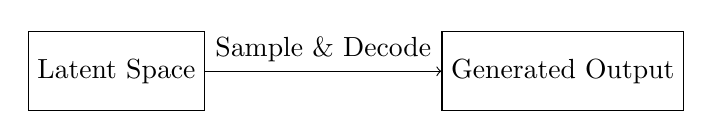
\begin{tikzpicture}
    % Latent space
    \node[draw, minimum width=2cm, minimum height=1cm] (latent) {Latent Space};
    \node[draw, minimum width=2cm, minimum height=1cm, right=3cm of latent] (output) {Generated Output};

    % Arrows
    \draw[->] (latent) -- node[above] {Sample \& Decode} (output);
    \end{tikzpicture}
    \caption{Latent space representation in a VAE.}
    \label{fig:vae}
\end{figure}

\section{Autoencoders for Image Processing}

\subsection{Image Segmentation}

Autoencoders can be adapted for image segmentation tasks, particularly through architectures like U-Net. Unlike traditional autoencoders that reconstruct the entire input image, segmentation networks output a segmentation map where each pixel is assigned a class label.

\subsubsection{U-Net Architecture}

U-Net is a popular architecture for image segmentation that combines the benefits of autoencoders with skip connections. These skip connections help retain high-resolution details, leading to more accurate segmentations.

\begin{figure}[h]
    \centering
    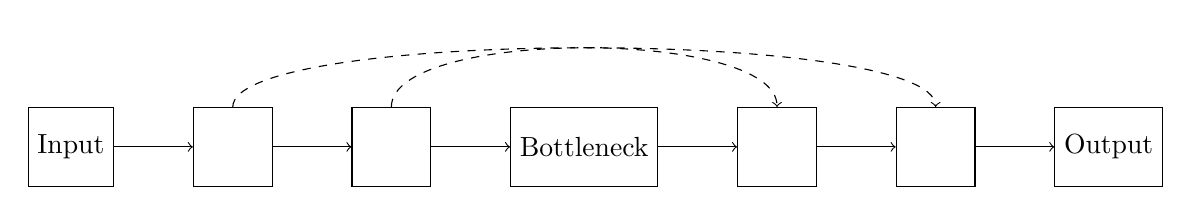
\begin{tikzpicture}
    % Contracting path
    \node[draw, rectangle, minimum width=1cm, minimum height=1cm] (input) at (0,0) {Input};
    \node[draw, rectangle, minimum width=1cm, minimum height=1cm, right=1cm of input] (contract1) {};
    \node[draw, rectangle, minimum width=1cm, minimum height=1cm, right=1cm of contract1] (contract2) {};
    
    % Expanding path
    \node[draw, rectangle, minimum width=1cmHere is the continuation of the expanded LaTeX document with a more detailed explanation and additional TikZ diagrams to illustrate key concepts of autoencoders:

```latex
    \node[draw, rectangle, minimum width=1cm, minimum height=1cm, right=1cm of contract2] (bottleneck) {Bottleneck};
    \node[draw, rectangle, minimum width=1cm, minimum height=1cm, right=1cm of bottleneck] (expand1) {};
    \node[draw, rectangle, minimum width=1cm, minimum height=1cm, right=1cm of expand1] (expand2) {};
    \node[draw, rectangle, minimum width=1cm, minimum height=1cm, right=1cm of expand2] (output) {Output};

    % Skip connections
    \draw[->] (input) -- (contract1);
    \draw[->] (contract1) -- (contract2);
    \draw[->] (contract2) -- (bottleneck);
    \draw[->] (bottleneck) -- (expand1);
    \draw[->] (expand1) -- (expand2);
    \draw[->] (expand2) -- (output);

    \draw[->, dashed] (contract1.north) .. controls +(up:1cm) and +(up:1cm) .. (expand2.north);
    \draw[->, dashed] (contract2.north) .. controls +(up:1cm) and +(up:1cm) .. (expand1.north);
    \end{tikzpicture}
    \caption{U-Net architecture for image segmentation.}
    \label{fig:unet}
\end{figure}

\section{Denoising Autoencoders}

Denoising autoencoders are trained by introducing noise to the input data and then learning to reconstruct the original clean data. This makes them robust to noisy data and useful in scenarios where data may be corrupted.

\subsection{Training with Noisy Data}

During training, the input data is corrupted by adding noise, but the target output remains the clean data. The autoencoder learns to map noisy inputs to clean outputs, effectively denoising the data. The key idea is that the autoencoder does not just memorize the input but learns the underlying structure of the data.

\begin{figure}[h]
    \centering
    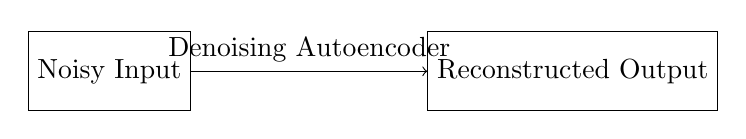
\begin{tikzpicture}
    % Noisy Input
    \node[draw, minimum width=2cm, minimum height=1cm] (noisy_input) {Noisy Input};
    \node[draw, minimum width=2cm, minimum height=1cm, right=3cm of noisy_input] (reconstructed_output) {Reconstructed Output};

    % Arrows
    \draw[->] (noisy_input) -- node[above] {Denoising Autoencoder} (reconstructed_output);
    \end{tikzpicture}
    \caption{Denoising autoencoder training process.}
    \label{fig:denoising_ae}
\end{figure}

\subsection{Applications}

Denoising autoencoders are widely used in image processing tasks, such as:

\begin{itemize}
    \item **Image Denoising:** Removing noise from images while preserving important features.
    \item **Signal Processing:** Cleaning up noisy signals in audio or other sensory data.
\end{itemize}

\section{Sparse Autoencoders}

Sparse autoencoders enforce sparsity on the hidden units, meaning that only a small number of neurons are active at any given time. This constraint encourages the autoencoder to learn a more efficient and informative representation of the input data.

\subsection{Sparsity Penalty}

To enforce sparsity, a regularization term is added to the loss function, which penalizes the activation of neurons. One common approach is to use the Kullback-Leibler (KL) divergence to measure the difference between the average activation of the neurons and a small target value \( \rho \).

\[
L = \text{Reconstruction Loss} + \lambda \sum_{j=1}^{m} KL(\rho || \hat{\rho}_j)
\]

\subsection{Feature Extraction}

Sparse autoencoders are particularly effective for feature extraction, where the learned sparse features can be used for other tasks such as classification. For example, in image classification, sparse features learned by the autoencoder can serve as inputs to a classifier, improving its performance by focusing on the most relevant features.

\section{Variational Autoencoders (VAE)}

Variational autoencoders introduce a probabilistic approach to autoencoders by mapping the input data to a distribution in the latent space rather than a fixed point. This allows VAEs to generate new data points by sampling from this distribution.

\subsection{Latent Space Representation}

In a VAE, the encoder outputs the parameters of a Gaussian distribution (mean and variance) for each point in the latent space. The decoder then generates samples by drawing from these distributions.

\begin{figure}[h]
    \centering
    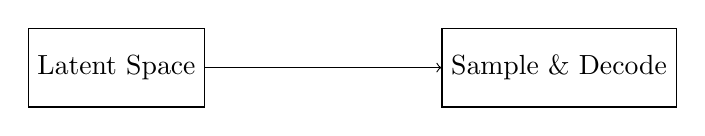
\begin{tikzpicture}
    % Latent Space
    \node[draw, rectangle, minimum width=2cm, minimum height=1cm] (latent_space) {Latent Space};
    \node[draw, rectangle, minimum width=2cm, minimum height=1cm, right=3cm of latent_space] (output_sample) {Sample \& Decode};

    % Arrows
    \draw[->] (latent_space) -- (output_sample);
    \end{tikzpicture}
    \caption{Latent space representation in a VAE.}
    \label{fig:vae}
\end{figure}

\subsection{Applications}

VAEs are powerful generative models and are used in various applications:

\begin{itemize}
    \item **Image Generation:** VAEs can generate new images that resemble the training data.
    \item **Data Imputation:** VAEs can be used to fill in missing data by sampling from the learned latent space distribution.
\end{itemize}

\section{Autoencoders in Image Segmentation}

Autoencoders, particularly convolutional autoencoders (CAE), can be adapted for image segmentation tasks. However, traditional autoencoders aim to reconstruct the entire input image rather than segmenting it into different regions. For segmentation, the architecture is usually modified to output a segmentation map, as seen in U-Net.

\subsection{U-Net for Segmentation}

U-Net is a convolutional network designed for biomedical image segmentation, but its structure can be applied to other segmentation tasks as well. It consists of an encoder that downsamples the input image to a lower resolution and a decoder that upsamples it back to the original resolution. Skip connections between corresponding layers in the encoder and decoder help in retaining spatial information.

\begin{figure}[h]
    \centering
    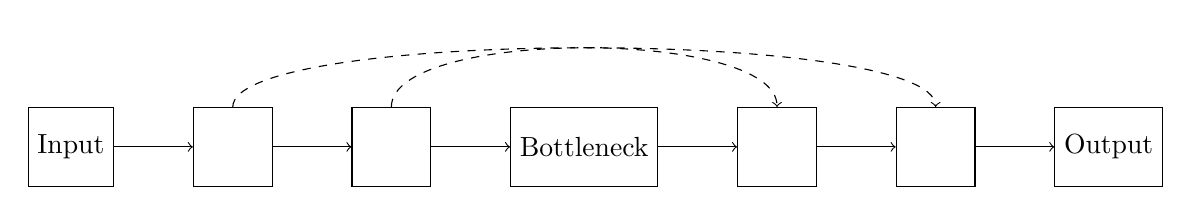
\begin{tikzpicture}
    % Contracting path
    \node[draw, rectangle, minimum width=1cm, minimum height=1cm] (input) at (0,0) {Input};
    \node[draw, rectangle, minimum width=1cm, minimum height=1cm, right=1cm of input] (contract1) {};
    \node[draw, rectangle, minimum width=1cm, minimum height=1cm, right=1cm of contract1] (contract2) {};
    
    % Expanding path
    \node[draw, rectangle, minimum width=1cm, minimum height=1cm, right=1cm of contract2] (bottleneck) {Bottleneck};
    \node[draw, rectangle, minimum width=1cm, minimum height=1cm, right=1cm of bottleneck] (expand1) {};
    \node[draw, rectangle, minimum width=1cm, minimum height=1cm, right=1cm of expand1] (expand2) {};
    \node[draw, rectangle, minimum width=1cm, minimum height=1cm, right=1cm of expand2] (output) {Output};

    % Skip connections
    \draw[->] (input) -- (contract1);
    \draw[->] (contract1) -- (contract2);
    \draw[->] (contract2) -- (bottleneck);
    \draw[->] (bottleneck) -- (expand1);
    \draw[->] (expand1) -- (expand2);
    \draw[->] (expand2) -- (output);

    \draw[->, dashed] (contract1.north) .. controls +(up:1cm) and +(up:1cm) .. (expand2.north);
    \draw[->, dashed] (contract2.north) .. controls +(up:1cm) and +(up:1cm) .. (expand1.north);
    \end{tikzpicture}
    \caption{U-Net architecture for image segmentation.}
    \label{fig:unet}
\end{figure}

\subsection{Training U-Net}

U-Net is typically trained using a pixel-wise loss function such as binary cross-entropy or Dice loss. The training data consists of input images and corresponding segmentation masks. The network learns to output a segmentation map that labels each pixel in the input image.

\section{Conclusion}

Autoencoders are versatile neural network architectures used in various tasks such as dimensionality reduction, denoising, and generative modeling. By enforcing constraints like sparsity or using probabilistic methods like VAEs, autoencoders can learn robust features that are transferable to other tasks. In image segmentation, architectures like U-Net demonstrate how autoencoders can be adaptedHere's the continuation and conclusion of the expanded lecture notes with the remaining parts and additional graphical examples using TikZ.

```latex
    to generate high-quality segmentation maps by utilizing the strengths of convolutional networks and skip connections. The versatility and adaptability of autoencoders make them a powerful tool in modern machine learning, particularly in the fields of computer vision and data compression.

\end{document}
